\documentclass[a4paper,12pt]{article} % тип документа

%  Русский язык
\usepackage[T2A]{fontenc}			% кодировка
\usepackage[utf8]{inputenc}			% кодировка исходного текста
\usepackage[english,russian]{babel}	% локализация и переносы

\usepackage{graphicx, scalerel}               % импорт изображений
\usepackage{wrapfig}                % обтекаемые изображения
\graphicspath{{pictures/}}          % обращение к подкаталогу с изображениями
\usepackage[14pt]{extsizes}         % для того чтобы задать нестандартный 14-ый размер шрифта
\usepackage{amsfonts}               % буквы с двойными штрихами
\usepackage[warn]{mathtext}         % русский язык в формулах
\usepackage{indentfirst}            % indent first
\usepackage[margin = 25mm]{geometry}% отступы полей
\usepackage{amsmath}                % можно выводить фигурные скобочки -- делать системы уравнений
\usepackage[table,xcdraw]{xcolor}   % таблицы
\usepackage{amsmath,amsfonts,amssymb,amsthm,mathtools} % Математика
\usepackage{wasysym}                % ???
\usepackage{upgreek}                % ???  
\usepackage{caption}
\usepackage{multirow}
\captionsetup{labelsep=period}
\usepackage{gensymb} % degree symbol


\begin{document}
	
	
	\begin{center}
		
		
		\textbf{НАЦИОНАЛЬНЫЙ ИССЛЕДОВАТЕЛЬСКИЙ УНИВЕРСИТЕТ \\ <<МОСКОВСКИЙ ФИЗИКО-ТЕХНИЧЕСКИЙ ИНСТИТУТ>>}
		\vspace{13ex}
		
		\textbf{Лабораторная работа 4.1.1\\ <<Центрированные оптические системы>>}
		\vspace{40ex}
		
		\normalsize{Овсянников Михаил Александрович \\ студент группы Б01-001\\ 2 курс ФРКТ\\}
	\end{center}
	
	\vfill 
	
	\begin{center}
		г. Долгопрудный\\ 
		2022 г.
	\end{center}
	
	
	\thispagestyle{empty} % выключаем отображение номера для этой страницы
	\newpage
	
	
	\textbf{Цель работы:} изучить центрированные оптические системы.
	
	\textbf{В работе используются:} оптическая скамья с набором рейтеров, положительные и отрицательные линзы, экран, осветитель с ирисовой диафрагмой, зрительная труба, светофильтры, кольцевые диафрагмы, линейка.
	
	\section*{Теоретические сведения}
	В большинстве реальных оптических систем содержится несколько преломляющих сферических поверхностей. Оптическую систему называют центрированной, если центры всех поверхностей лежат на одной прямой, которую называют главной оптической осью системы. В предлагаемой работе изучаются методы определения фокусных расстояний тонких собирающих и рассеивающих линз; определяются характеристики сложной системы, составленной из тонких линз; исследуются недостатки реальных линз — сферические и хроматические аберрации или отклонение световых лучей от гомоцентричности.
	
	\subsection*{А. Определение фокусных расстояний положительных и отрицательных линз и положений главных плоскостей сложной оптической системы}
	
	Идеальной оптической системой называют систему, в которой сохраняется гомоцентричность пучков и изображение геометрически подобно предмету. Идеальная оптическая система обладает осью симметрии, которая называется главной оптической осью.
	
	Оптическая система называется положительной или собирающей, если лучи, падающие на неё параллельно главной оптической оси, пройдя систему, отклоняются в направлении оси — собираются. Если ввести расстояния от предмета и изображения до соответствующих главных плоскостей, то легко установить соотношение между этими расстояниями и фокусным расстоянием системы:
	
	\begin{equation*}
		\frac{1}{a_1} + \frac{1}{a_2} = \frac{1}{f}
	\end{equation*}

	В формуле $a_1$ считается положительным, если предмет лежит слева от передней главной плоскости, $a_2$ положительно, если изображение лежит справа от задней плоскости, а фокусное расстояние $f$ берётся со своим знаком.
	
	\newpage
	\begin{center}
		I. Определение фокусного расстояния тонкой положительной линзы
	\end{center}
	
	\begin{figure}[h!]
		\centering
		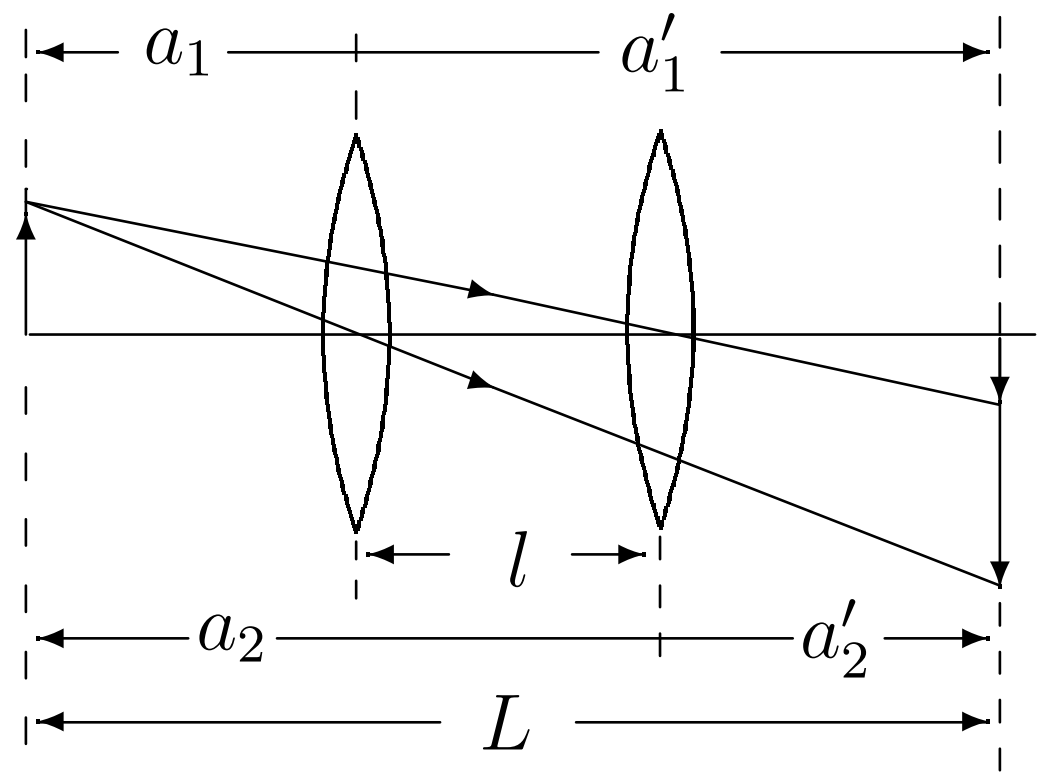
\includegraphics[scale=0.6]{Pictures/Бессель}
		\caption{Определение фокусного расстояния методом Бесселя}
	\end{figure}

	\textit{Способ 1}. Пусть расстояние между предметом и экраном превышает $4f$. Нетрудно убедиться, что при этом всегда найдутся два таких положения линзы, при которых на экране получаются отчётливые изображения предмета (в одном случае уменьшенное, в другом — увеличенное). Из соображений симметрии ясно, что $a_1 = a_2'$ и $a_2 = a_1'$ (рис. 1). Обозначая расстояние между предметом и экраном через $L$, а расстояние между двумя положениями линзы через $l$, получим: $L = a_1 + a_2$; $l = a_2 - a_1 = a_1' - a_2'$. Отсюда:
	\begin{equation*}
		a_1 = \frac{L - l}{2}; \;\;\; a_1' = \frac{L+l}{2}
	\end{equation*}
	
	Подставляя это в формулу линзы, найдём после несложных преобразований:
	
	\begin{equation*}
		f = \frac{L^2 - l^2}{4L}.
	\end{equation*}
	
	\newpage
	\textit{Способ 2}. Фокусное расстояние тонкой положительной линзы можно определить с помощью зрительной трубы, настроенной на бесконечность, то есть на параллельный пучок лучей. Разместив между предметом и зрительной трубой положительную линзу и перемещая её вдоль оси системы, можно найти резкое изображение предмета в окуляре зрительной трубы. При этом расстояние от середины линзы до предмета равно фокусному расстоянию тонкой линзы. Для толстой линзы зрительная труба позволяет определить только положение главного фокуса.
	

	\begin{center}
		II. Определение фокусного расстояния тонкой отрицательной линзы
	\end{center}

	\begin{figure}[h!]
		\centering
		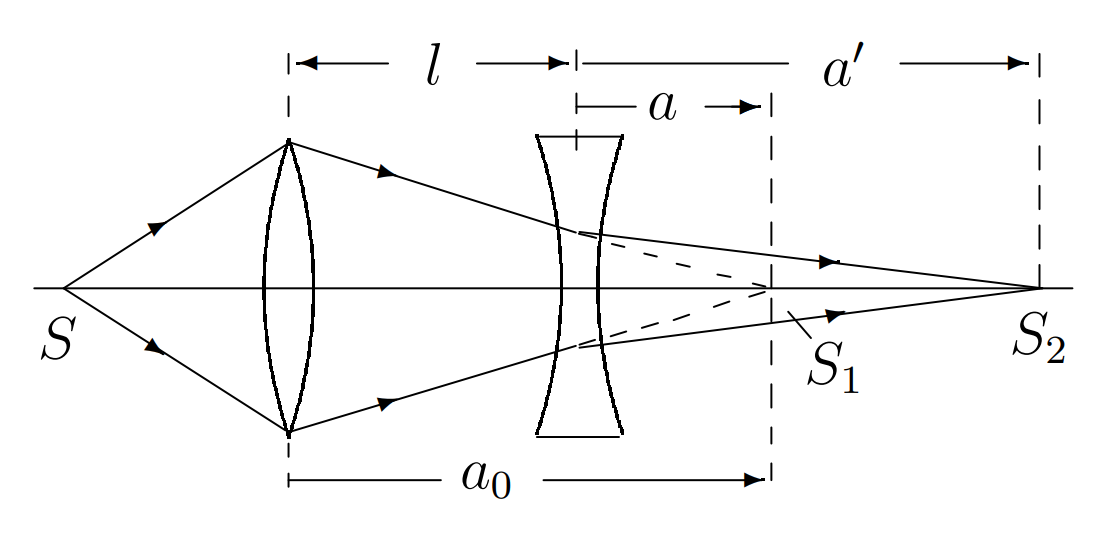
\includegraphics[scale=0.6]{Pictures/Отрицат}
		\caption{Определение фокусного расстояния отрицательной линзы}
	\end{figure}

	\textit{Способ 1}. Определение фокусного расстояния отрицательной линзы затруднено тем, что изображение предмета получается мнимым и поэтому не может быть получено на экране. Эту трудность легко обойти с помощью вспомогательной положительной линзы.
	
	Сначала с помощью положительной линзы получают на экране действительное изображение предмета $S$ (точка $S_1$ на рис. 2). Затем на пути лучей, выходящих из положительной линзы, располагают исследуемую отрицательную линзу и, отодвигая экран, получают четкое изображение предмета на экране, образованное двумя линзами. Точка $S_1$ пересечения сходящихся лучей играет по отношению к отрицательной линзе роль мнимого источника. Изображение источника переместится теперь в точку $S_2$. Определив расстояния $a = a_0 - l$ и $a'$, рассчитывают фокусное расстояние рассеивающей линзы по формуле тонкой линзы.
	
	\newpage
	\textit{Способ 2}. Если расстояние $a$ (рис. 2) совпадает с фокусным расстоянием отрицательной линзы, то изображение перемещается в бесконечность, т. е. лучи выходят из линзы параллельным пучком. Параллельность пучка можно установить с помощью зрительной трубы, настроенной на бесконечность. Зная расстояние от первой линзы до точки $S_1$ и расстояние между линзами, нетрудно определить фокусное расстояние тонкой отрицательной линзы. Для толстой отрицательной линзы этот метод позволяет определить только положение главного фокуса.
	
	\begin{center}
		III. Определение фокусного расстояния и положения главных плоскостей сложной оптической системы
	\end{center}
	
	Ни один из описанных выше способов не позволяет определить фокусное расстояние и положение главных плоскостей толстой линзы, т. е. такой оптической системы, толщина которой не мала по сравнению с фокусным расстоянием.
	
	\begin{figure}[h!]
		\centering
		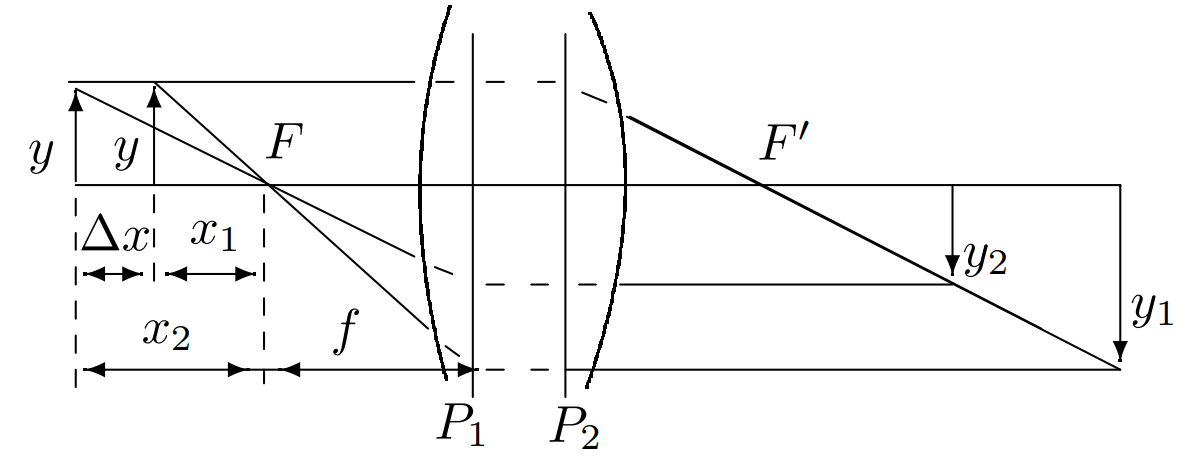
\includegraphics[scale=0.6]{Pictures/Сложн}
		\caption{Сложная оптическая система}
	\end{figure}
	
	Фокусное расстояние толстой положительной линзы определяют по методу Аббе (рис. 3). Пусть предмет, линейный размер которого равен $y$, находится на расстоянии $x_1$ от главного фокуса $F$ положительной оптической системы. Изображение предмета имеет размер $y_1$. Линейное увеличение $\Gamma_1 = \frac{y_1}{y} = \frac{f}{x_1}$. Если теперь отодвинуть предмет от линзы на расстояние $\Delta x$, то линейное увеличение $\Gamma_2 = \frac{y_2}{y} = \frac{f}{x_2}$.
	
	Нетрудно получить:
	\begin{equation*}
		f = \frac{\Delta x}{1/\Gamma_1 - 1/\Gamma_2}.
	\end{equation*}

	\newpage
	Теоретически фокусное расстояние $f'$ сложной системы, состоящей из двух тонких положительных линз, можно рассчитать, если известны фокусные расстояния каждой линзы и расстояние между их центрами $l_{12}$:
	\begin{equation*}
		\frac{1}{f'} = \frac{1}{f_1'} + \frac{1}{f_2'} - \frac{|l_{12}|}{f_1'f_2'}.
	\end{equation*}

	\subsection*{Б. Аберрации реальных оптических систем}
	
	\subsubsection*{Сферическая}
	Сферическая аберрация возникает при преломлении широких (не параксиальных) пучков света на сферических поверхностях линз. Рисунок 4 поясняет возникновение сферической аберрации.
	
	\begin{figure}[h!]
		\centering
		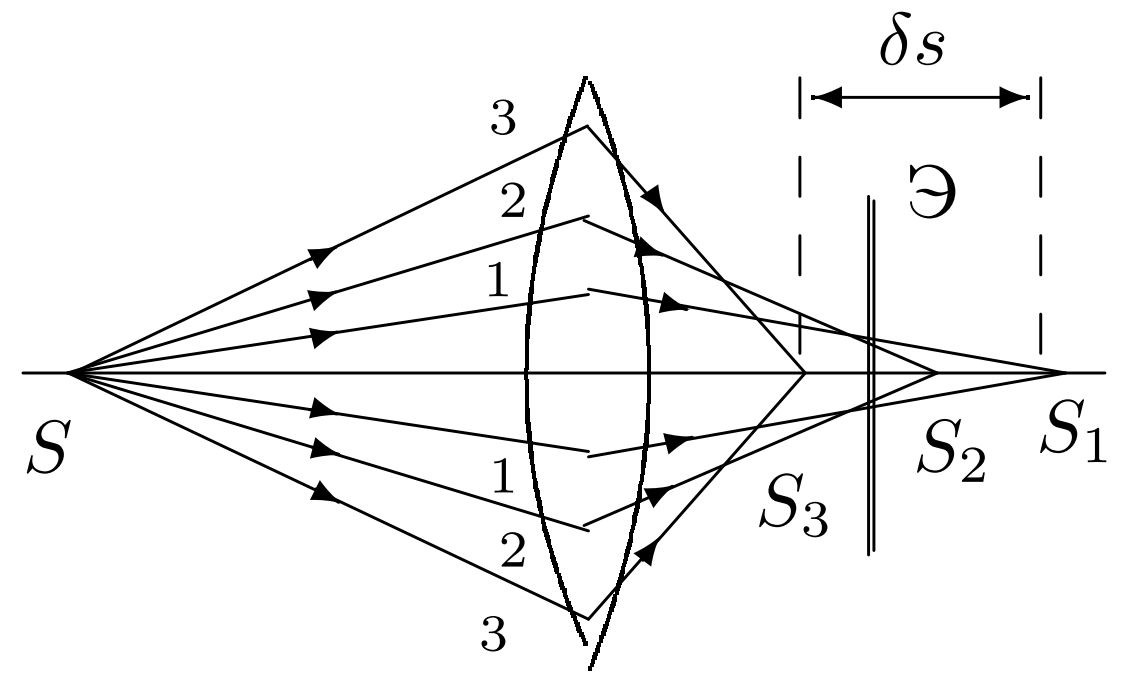
\includegraphics[scale=0.5]{Pictures/Сфер}
		\caption{Сферическая аберрация}
	\end{figure}

	Для лучей, проходящих на расстоянии $h$ от центра линзы, расстояние $s$ выражается соотношением:
	\begin{equation*}
		s = \frac{R}{n - 1}\left(1 - \frac{1}{2} \frac{n^2 h^2}{R^2}\right).
	\end{equation*}

	Характеристической кривой сферической аберрации называют зависимость 
	\begin{equation*}
		\delta s(h) = s(h) - s(0) = -\frac{1}{2}\frac{n^2 h^2}{(n - 1)R} = -\frac{1}{2}\left(\frac{n}{n - 1}\right)^2 \left(\frac{h}{f}\right)^2 f.
	\end{equation*}

	При $h = r$ — радиус линзы, формула определяет продольную сферическую аберрацию линзы.
		
	
	\subsubsection*{Хроматическая}
	Хроматическая аберрация (зависимость фокусного расстояния линзы от длины волны) возникает вследствие дисперсии показателя преломления стёкол, т. е. из-за того, что показатель преломления $n = n(\lambda)$. Возникновение хроматической аберрации поясняет рис. 5.
	
	\begin{figure}[h!]
		\centering
		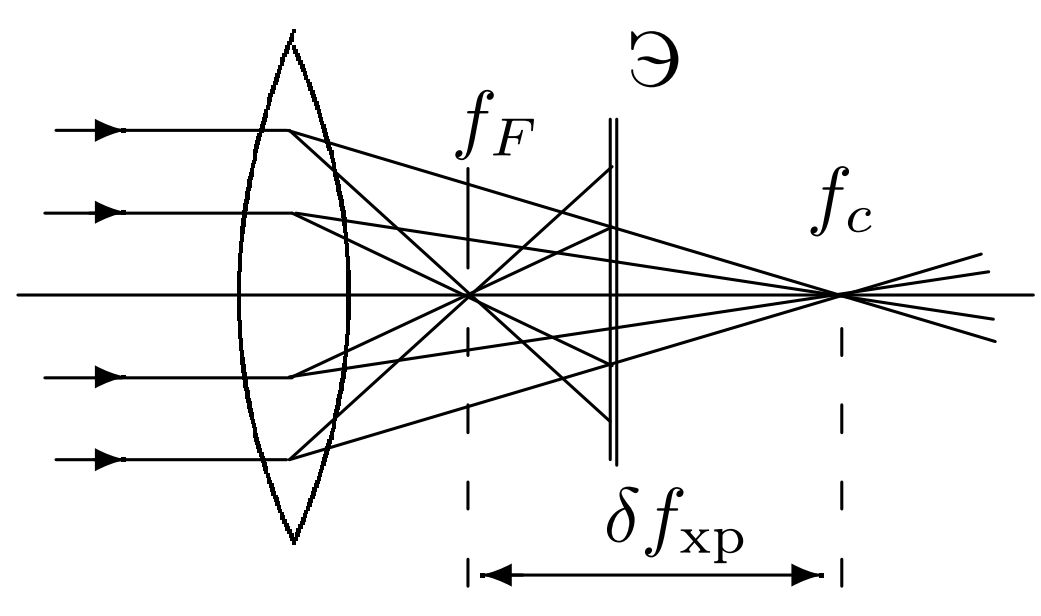
\includegraphics[scale=0.6]{Pictures/Хром}
		\caption{Хроматическая аберрация}
	\end{figure}

	Хроматическую аберрацию принято характеризовать разностью фокусных расстояний для двух характерных спектральных
линий водорода, расположенных в крайних частях видимой области спектра: $\lambda_F$ = 486,1 нм (голубая линия $F$ водорода), $\lambda_C$ = 656,3 нм (красная линия $C$ водорода):
	\begin{equation*}
		\delta f_{\text{хр}} = f_F - f_C.
	\end{equation*}	

	Для характеристики дисперсионных свойств стёкол часто пользуются так называемым коэффициентом дисперсии, или числом Аббе:
	\begin{equation*}
		\nu = \frac{n_D - 1}{n_F - n_C},
	\end{equation*}

	где $n_D$ - показатель преломления для жёлтой линии $D$ натрия $\lambda_D$ = 589,3 нм.
	Тогда:
	
	\begin{equation*}
		\delta f_{\text{хр}} = -\frac{1}{\nu} f_D.
	\end{equation*}

	\newpage
	\section*{Ход работы}
	\subsection*{A. Определение фокусных расстояний положительных и отрицательных линз и положений главных плоскостей сложной оптической системы}
	
	\begin{center}
		\textbf{Центрировка элементов оптической системы}
	\end{center}

	\begin{enumerate}
		\item Из имеющегося набора отберем собирающие линзы: 
		
		$\bullet \; F_1 \approx 90$ мм - собирающая
		 
		$\bullet \; F_2 \approx 100$ мм - собирающая	

		$\bullet \; F_3 = 70$ мм - собирающая
		
		$\bullet \; F_4$ - рассеивающая.
		
		
		\item Соберем и отцентрируем установку.
		
		\item Отодвинем экран от осветителя и разместим в промежутке рейтер с собирающей линзой № 1. Передвигая линзу и экран вдоль скамьи, добьемся четкого изображения края ирисовой диафрагмы осветителя на экране. Закрепим рейтеры. Смещая линзу с помощью поперечных салазок и по высоте, приведем центр изображения к центру экрана.
		
		\item Оптические оси линз устанавливаем параллельно ребру оптической скамьи на глаз.
		
		\item Для центрировки рассеивающих линз воспользуемся уже отцентрированной положительной линзой, расположив её впереди отрицательной.
		
	\end{enumerate}


	\begin{center}
	\textbf{I. Определение фокусного расстояния тонкой положительной линзы}
	\end{center}
	
	\textit{Способ 1 (метод Бесселя):}
	\begin{enumerate}
		\item Установим положительную линзу № 1 между осветителем и экраном. Расположим экран на расстоянии $L > 4f$ от предмета (рис. 1). Перемещая линзу вдоль скамьи, получим увеличенное и уменьшенное изображения предмета на экране.
		
		\item С помощью линейки измерьте расстояния от линзы до предмета и до изображения ($a_1$, $a_2$, $a_1'$, $a_2'$ на рис. 1). Рассчитаем фокусное расстояние линзы, проделав эксперимент несколько раз.
		
		$\bullet \;$ $L = 55$ см, $a_1 = 44,5$ см, $a_1' = 10,5$ см, $a_2 = 11$ см, $a_2' = 44$ см.
		
		Откуда получаем $l = (33,5 \pm 0,2)$ см.
		
		И фокусное расстояние:
		\begin{equation*}
			f = \frac{L^2 - l^2}{4L};
		\end{equation*}
	
		\begin{eqnarray*}
			\sigma_f = \delta_f f = f \delta_{\frac{L^2 - l^2}{L}} = f \sqrt{\delta_{L^2 - l^2}^2 + \delta_L^2} = f\sqrt{\frac{\sigma_{L^2 - l^2}^2}{(L^2 - l^2)^2} + \delta_L^2} = \\
			 = f\sqrt{\frac{\sigma_{L^2}^2 + \sigma_{l^2}^2}{(L^2 - l^2)^2} + \delta_L^2} = f\sqrt{\frac{(2\sigma_{L}L)^2 + (2\sigma_{l}l)^2}{(L^2 - l^2)^2} + \frac{\sigma_L^2}{L^2}} = \\ 
			 f\sqrt{\frac{(2\sigma_{L}L)^2 + (2\sqrt{2}\sigma_{L}l)^2}{(L^2 - l^2)^2} + \frac{\sigma_L^2}{L^2}}
			 = f \sigma_L \sqrt{\frac{4L^2 + 8l^2}{(L^2 - l^2)^2} + \frac{1}{L^2}}
		\end{eqnarray*}
		
		Итого:
		
		\begin{equation*}
			f = (8,65 \pm 0,08) \text{ см}.
		\end{equation*}
		
		Повторим опыт еще раз.
		
		$\bullet \;$ $L = 79$ см, $a_1 = 14$ см, $a_1' = 65$ см, $a_2 = 67,5$ см, $a_2' = 11,5$ см.
		
		В этот раз:
		\begin{equation*}
			f = (10,7 \pm 0,1) \text{ см}.
		\end{equation*}
	
		И в последний раз.
		
		$\bullet \;$ $L = 72,5$ см, $a_1 = 14,5$ см, $a_1' = 58$ см, $a_2 = 60$ см, $a_2' = 12,5$ см.
		
		Получилось:
		\begin{equation*}
			f = (11,0 \pm 0,1) \text{ см}.
		\end{equation*}
	
		В итоге получаем такое вот значение:
		\begin{equation*}
			\boxed{f = (10,2 \pm 0,2) \text{ см}}
		\end{equation*}
	
		\newpage
		\textit{Способ 2 (по зрительной трубе):}
		\item Настроим трубу на бесконечность.
		
		\item Поставим положительную линзу на расстоянии от предмета примерно равном фокусному. На небольшом расстоянии от линзы закрепим трубу, настроенную на бесконечность, и отцентрируем её по высоте. Передвигая линзу вдоль скамьи, сначала получим в окуляре зрительной трубы изображение поверхности матового стекла; затем, перемещая линзу с помощью поперечных салазок и меняя диаметр светового пятна с помощью ирисовой диафрагмы, настроимся на четкое изображение края диафрагмы. При этом расстояние между предметом и серединой тонкой линзы (между проточками на оправах) равно фокусному. После всего этого повернем линзу другой стороной и повторим эксперимент.
		
		\vspace{5mm}
		Тогда:
		
		$\bullet$ Одна сторона: $\;\;\; f = (10,0 \pm 0,1)$ см.
		
		$\bullet$ Другая сторона: $f = (10,5 \pm 0,1)$ см.
		
		Следовательно, линзу можно с хорошей точностью считать идеальной.
		
		\item Повторим все это с линзой №2:
		
		$\bullet$ Одна сторона: $\;\;\; f = (13,0 \pm 0,1)$ см.
		
		$\bullet$ Другая сторона: $f = (13,5 \pm 0,1)$ см.
		
		Значит, и вторую линзу тоже можно считать идеальной.
	
	\end{enumerate}


	\begin{center}
		\textbf{II. Определение фокусного расстояния тонкой отрицательной линзы}
	\end{center}
	\textit{Способ 1:} 
	\begin{enumerate}
		\item Для определения фокусного расстояния тонкой отрицательной линзы используем вспомогательную положительную линзу. Сначала с помощью положительной линзы №1 получим на экране увеличенное изображение предмета и измерим линейкой расстояние от линзы до экрана ($a_0$ на рис. 2). Затем между положительной линзой и экраном разместим рассеивающую линзу и, отодвигая экран от линзы, найдем действительное изображение предмета, образованное системой линз. Измерим расстояние $a'$ от рассеивающей линзы до экрана и расстояние между линзами $l$.
		
		Получаем следующее:
		
		$a_0 = (320 \pm 1)$ мм;	 $\hspace{10mm} l = (230 \pm 1)$ мм;  $\hspace{10mm} a' = (580 \pm 1)$ мм.
		
		
		Рассчитаем величину $a = a_0 - l$ и определим фокусное расстояние рассеивающей линзы с помощью формулы тонкой линзы:
		
		$a = (90 \pm 2)$ мм.
		
		\begin{equation*}
			f = \frac{a \cdot a'}{a - a'}; \hspace{5mm} \sigma_f = |f| \sqrt{\delta_{aa'}^2 + \delta_{a - a'}^2} = |f| \sqrt{\delta_a^2 + \delta_{a'}^2 + \frac{\sigma_a^2 + \sigma_{a'}^2}{(a - a')^2}}
		\end{equation*}
	
		Вычисляем:
		
		\begin{equation*}
			\boxed{f = (-10,7 \pm 0,2) \text{ см}}
		\end{equation*}
	
	\textit{Способ 2 (по зрительной трубе):}
	
	\item Для определения фокусного расстояния тонкой отрицательной линзы используем схему, изображённую на рис. 2. Сначала получим на экране увеличенное изображение диафрагмы при помощи положительной линзы №1. Измерим расстояние $a_0$ между линзой и экраном.
	
	Разместим сразу за экраном трубу, настроенную на бесконечность, и закрепим её. Уберем экран и поставим на его место исследуемую рассеивающую линзу. Отцентрируем световой пучок с помощью листа бумаги. Перемещая рассеивающую линзу, найдем в окуляре зрительной трубы резкое изображение края диафрагмы.
	
	Измерив расстояние между линзами $l$, рассчитаем фокусное расстояние рассеивающей линзы: $f = a_0 - l$.
	
	После всего этого повторим опыт, предварительно перевернув линзу другой стороной. Получаем такие результаты:
	
	$\bullet$ Одна сторона: 
	
	$a_0 = (370 \pm 1)$ мм; $l = (260 \pm 1)$ мм $\Longrightarrow f = (-11,0 \pm 0,5)$ см.
	
	$\bullet$ Другая сторона:
	
	$a_0 = (370 \pm 1)$ мм; $l = (260 \pm 1)$ мм $\Longrightarrow f = (-11,0 \pm 0,5)$ см.
	

	\vspace{5mm}	
	Как видно, значения совпадают. Вдобавок, они сходятся со значением, найденным первым способом.
	\end{enumerate}

	\newpage
	\begin{center}
		\textbf{III. Определение фокусного расстояния и положения главных плоскостей сложной оптической системы}
	\end{center}

	\begin{enumerate}
		\item Для создания сложной оптической системы установим в центре оптической скамьи две тонких собирающих линзы на расстоянии, сблизив их на минимальное расстояние -- до соприкосновения рейтеров. Закрепим рейтеры и измерим расстояние $l_{12}$ между центрами линз: $l_{12} = (5,5 \pm 0,1)$ см.
		
		Для определения фокусного расстояния системы методом Аббе расположим экран на дальнем конце скамьи.
		
		Перемещая осветитель вдоль скамьи, получим на экране резкое изображение. 
		
		Отодвинем источник на несколько сантиметров и, передвигая экран, снова получим резкое изображение. Зарегистрируем перемещения предмета $\Delta x$ и его изображения $\Delta x'$, а также размеры изображений:
		
		$\bullet \;\Delta x = (-30 \pm 1)$ мм; $\hspace{6mm} \Delta x' = (-400 \pm 1)$ мм;
		
		$\bullet \;y_1 = (150 \pm 1)$ мм;  $\hspace{10mm} y_2 = (35 \pm 1)$ мм.
		
		$\bullet \;y = (20 \pm 1)$ мм -- размер предмета.
		
		Рассчитаем фокусное расстояние системы:
		\begin{equation*}
			f_\Sigma^\text{эксп} = \frac{\Delta x}{y/y_1 - y/y_2} = (6,9 \pm 0,3) \text{ см}.
		\end{equation*}
	
		\begin{equation*}
			f_\Sigma^\text{эксп} = -\frac{\Delta x'}{y_1/y - y_2/y} = (7,0 \pm 0,1) \text{ см}.
		\end{equation*}
	
		\begin{equation*}
			f_\Sigma^\text{теор} = -\frac{1}{\frac{1}{f_1} + \frac{1}{f_2} - \frac{|l_{12}|}{f_1f_2}} = (7,4 \pm 0,1) \text{ см}.
		\end{equation*}
		
		Легко видеть, что получившиеся результаты достаточно близки друг к другу.
		
		\item Для нахождения положения главных фокусов системы закрепим зрительную трубу за второй линзой, подвинем осветитель к первой линзе и отцентрируем систему с помощью листа бумаги. Медленно отодвигая осветитель от системы, сначала найдем резкое изображение поверхности стекла в окуляре зрительной трубы, а затем, последовательно уменьшая размер пятна и перемещая пятно с помощью винта поперечных салазок линзы, настроимся на край ирисовой диафрагмы.
		
		Определим положение переднего главного фокуса системы, измерив расстояние от предмета до первой линзы: $F_{1\Sigma} = (50 \pm 1)$ мм.
		
		\item Поменяв линзы местами и проделав ту же процедуру, найдем задний главный фокус системы: $F_{2\Sigma} = (45 \pm 1)$ мм.
	\end{enumerate}

	\subsection*{Б. Аберрации реальных оптических систем}
	
	\begin{center}
		\textbf{I. Сферическая аберрация}
	\end{center}

	\begin{enumerate}
		\item Для качественного наблюдения сферической аберрации расположим осветитель и экран на дальних концах скамьи. Установим линзу № 3 на расстоянии $a_1$ от предмет а чуть большем фокусного и наденем на неё маску минимального размера. Перемещая линзу, получим на удаленном экране резкое изображение ирисовой диафрагмы осветителя. Установим маску максимального диаметра и убедимся, что при неизменном расстоянии $a_1$ расстояние $a_2$ от линзы до изображения заметно изменилось.
		
		\item Для количественной оценки аберраций установим нониусную шкалу продольного перемещения линзы на 0. Используя зрительную трубу, получим параллельный пучок от линзы для параксиальных лучей и запишем отсчёт по нониусной шкале линзы. Далее значения представлены уже относительно нового начала. 
		
		Увеличивая диаметр маски и подстраиваясь к новому положению фокуса при помощи нониусного винта, будем отмечать соответствующие отсчёты по нониусной шкале.
		
		Получаем следующие данные:
		
		\begin{table}[h!]
			\centering
			\begin{tabular}{|c|c|}
				\hline
				$h$, мм & $|\delta s|$, см \\ \hline
				5       & 0,3            \\ \hline
				10      & 0,6            \\ \hline
				20      & 2,3            \\ \hline
			\end{tabular}
		\caption{Зависимость $\delta s(h)$}
		\end{table}
	
		Построим график зависимости $|\delta s(h^2)|$:
		\newpage
		
		\begin{figure}[h!]
			\centering
			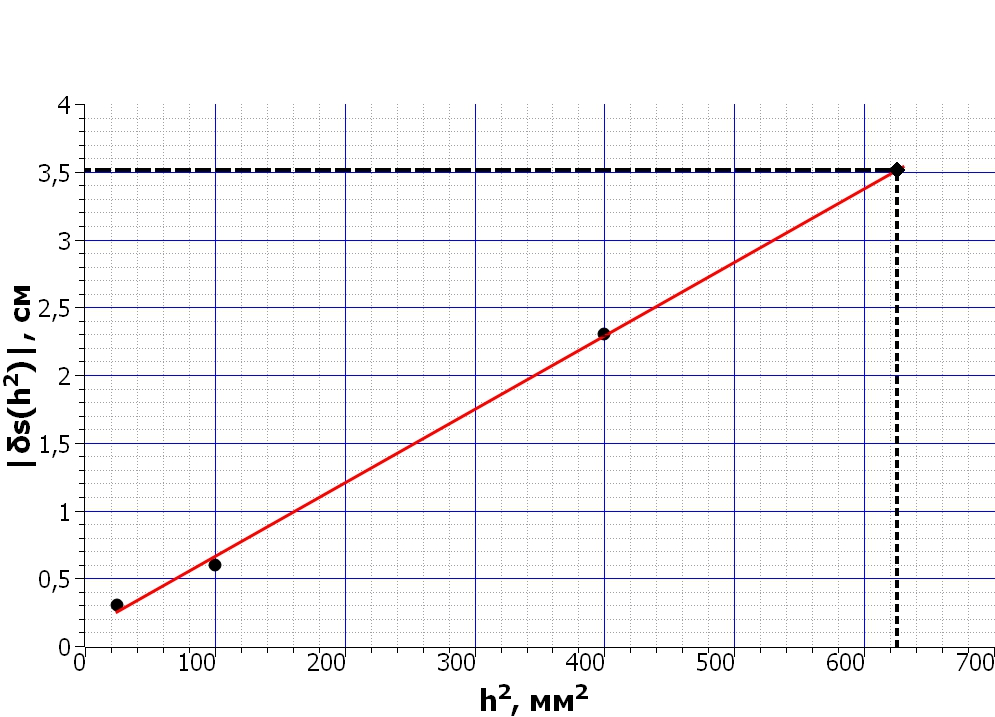
\includegraphics[scale=0.7]{Pictures/d(h)}
			\caption{Зависимость $|\delta s(h^2)|$}
		\end{figure}
	
		Видно, что точки хорошо укладываются на прямую.
		
		Экстраполируем к $h = r = 2,5$ см -- радиус линзы -- получаем продольную аберрацию линзы:
		\begin{equation*}
			|\delta s(r)| = |s(r) - s(0)| = (3,5 \pm 0,2)\text{ см}.
		\end{equation*}
	
		А по наклону прямой найдем показатель преломления:
		\begin{equation*}
			|\delta s| = \frac{1}{2}\left(\frac{n}{n - 1}\right)^2\frac{1}{f} \cdot h^2 = kh^2.
		\end{equation*}
		
		Из графика имеем: $k = (5,4 \pm 0,3)\cdot 10^{-2} \text{ мм}^{-1}$.
		
		Отсюда выходит: 
		\begin{equation*}
			\boxed{n = (1,57 \pm 0,03)}
		\end{equation*}

		
	\end{enumerate}

	\begin{center}
		\textbf{II. Хроматическая аберрация}
	\end{center}

	\begin{enumerate}
		\item Используя зрительную трубу и три светофильтра (красный($C$), жёлтый($D$) и синий($F$)), определим по нониусной шкале положения плосковыпуклой линзы, соответствующие резкому изображению диафрагмы при каждом из цветов:
		
		$f_C = (70,7 \pm 0,1)$ мм; $f_D = (70,3 \pm 0,1)$ мм; $f_F = (69,4 \pm 0,1)$ мм.
	
		\item Рассчитаем хроматическую аберрацию:
		\begin{equation*}
			\delta f_{\text{хр}} = f_F - f_C = (-1,3 \pm 0,2) \text{ мм}.
		\end{equation*}
	
		Вычислим число Аббе:
		\begin{equation*}
			\nu = -\frac{f_D}{\delta f_{\text{хр}}} = (55 \pm 6).
		\end{equation*}
	
		По диаграмме Аббе это соответствует кронам как сорту стекла.
	\end{enumerate}
	
	
	\section*{Вывод}
	В работе были изучены центрированные оптические системы. Были определены фокусные расстояния линз:
	
	$\bullet \; F_1 = (10,2 \pm 0,2)$ см - собирающая;

	$\bullet \; F_2 = (13,3 \pm 0,3)$ см - собирающая;

	$\bullet \; F_4 = (-10,7 \pm 0,2)$ см - рассеивающая.
	
	Мы пронаблюдали явления аберраций оптической системы такие как сферическая и хроматическая аберрации. Было найдено значение продольной аберрации линзы: $|\delta s(r)| = (3,5 \pm 0,2)$ см.
	
	Помимо этого еще было получено значение хроматической аберрации: $\delta f_{\text{хр}} = (-1,3 \pm 0,2)$ мм, и число Аббе: $\nu = (55 \pm 6)$, что позволяет заключить, что стекло сделано из сорта крон. Все ошибки связаны с неточностью измерений.


\end{document}